\documentclass[11pt, a4paper]{article}
\usepackage{amsmath, amssymb, amsbsy}
\usepackage[amsmath, thmmarks]{ntheorem}
\usepackage{algorithm}
\usepackage{algpseudocode}
\usepackage{xcolor}
\usepackage{tikz}
\usepackage{paralist}
\usepackage{nicefrac}
% =========== 


% ============================= Pseudocode Customization =======================
% Packages: algorithm, algpseudocode.
\algrenewcommand{\algorithmicrequire}{\textbf{Input:}}
\algrenewcommand{\algorithmicensure}{\textbf{Output:}}
\algnewcommand\algorithmicto{\textbf{to} } % a trailing space is needed.
\algnewcommand\algorithmicbreak{\textbf{break}} % break keyword.
\newcommand{\breakif}[1]{\State \textbf{if} {#1} \textbf{then break}}


% ============================= Math Theorem Envs ==============================
\theorembodyfont{\normalfont}
\newtheorem{df}{Definition}[section]
\newtheorem{thm}[df]{Theorem}
\newtheorem{eg}[df]{Example}
\newtheorem{prop}[df]{Proposition}
\newtheorem{lem}[df]{Lemma}
\newtheorem{cor}[df]{Corollary}
\newtheorem{re}[df]{Remark}

% Customize proof env.
\theoremstyle{nonumberplain} % no numbering
\theoremsymbol{$\square$}    % proof end with square.
\newtheorem{pf}{Proof}


% =============================== Operators ====================================
\DeclareMathOperator{\ent}{Entropy}
\DeclareMathOperator*{\p}{\mathbb{P}} % probability.
\DeclareMathOperator{\sign}{sign}
\DeclareMathOperator*{\argmax}{argmax}
\DeclareMathOperator*{\argmin}{argmin}
\DeclareMathOperator*{\E}{\mathbb{E}} % Expectation.
\DeclareMathOperator{\dist}{dist} % distance.
\DeclareMathOperator{\indi}{\mathbb{I}}
\DeclareMathOperator{\tr}{tr} % trace of an matrix.


% =============================== New Commands =================================
% Logical connectives:
\newcommand{\OR}{\textbf{OR} } % a space is needed here.
\newcommand{\AND}{\textbf{AND} } 
\newcommand{\XOR}{\textbf{XOR} } 

% Math commands:
\newcommand{\T}[1]{\ensuremath{{#1}^\mathsf{T}}} % Matrix transposition.
\newcommand{\inv}[1]{\ensuremath{{#1}^{-1}}} % Inversion.
\newcommand{\V}[1]{\ensuremath{\boldsymbol{#1}}}

% Shorthand commands:
\newcommand{\hypo}[1]{\ensuremath{{#1}: \mathcal{X} \longrightarrow \mathcal{Y}}} % Hypothesis function.
\newcommand{\dataset}{\ensuremath{D = \{(\V{x}_1, y_1), \ldots, (\V{x}_m, y_m)\}}} % Labeled training set.
\newcommand{\st}{\text{s.t.\ }}
\newcommand{\magenta}[1]{\textcolor{magenta}{#1}} % turn the color of text into magenta.
\newcommand{\hl}[2][yellow]{\colorbox{#1}{#2}} % highlight the text.
\newcommand{\pfrac}[2]{\ensuremath{\frac{\partial {#1}}{\partial {#2}}}}

% =====================================================
\numberwithin{equation}{section}

% =============================== Document =====================================
\begin{document}

% ========Linear Models================
\section{Linear Models}
hahaha

% ========Decision Trees===============
\section{Decision Trees}
Decision Tree.

% Pseudocode of decision tree algorithm.
\begin{algorithm}
    \caption{Decision Tree}\label{decision_tree}
    \begin{algorithmic}[1]
        \Require training set $D = \{(x_1, y_1), (x_2, y_2), \ldots, (x_m, y_m)
        \}$; attribute set $A = \{a_1, a_2, \ldots, a_d\}$.
        \Ensure a decision tree.
        \Procedure{DT}{$D, A$}
            \State Generate a node.
            \If{$y_i = c, \forall i = 1, \ldots, m$} \Comment{All samples have 
            the same label}
                \State mark the node as a leaf with label $c$; \Return
            \EndIf
            \If{$A = \emptyset$ \OR samples of $D$ take the same value on each
            attribute from $A$}\Comment{attributes from $A$ cannot distinguish
            elements of $D$}
                \State mark the node as a leaf with the majority label of $D$; 
                \Return
            \EndIf
            \State Choose the \textit{best} attribute $a_*$ from $A$.\label{measurement}
            \ForAll{possible value $a_*^v$ of $a_*$}
                \State generate a branch from node.
                \State let $D_v$ be all samples that take value $a_*^v$ on attribute
                $a_*$.
                \If{$D_v = \emptyset$} \Comment{no sample of $D$ takes value $a_*^v$
                on $a_*$}
                    \State mark the branch as a leaf with the majority label of 
                    $D$; \Return
                \Else
                    \State set the branch to \Call{DT}{$D_v, A-\{a_*\}$}.
                \EndIf
            \EndFor
        \EndProcedure
    \end{algorithmic}
\end{algorithm}



% ========SVM========================
\section{Support Vector Machine}
Let \dataset\ be the training set where $y_i \in\{-1, +1\}$. The SVM is an algorithm that tries to find a 
hyperplane $y = \langle\V{w}, \V{x}\rangle + b$ which separate the positive examples from the negative ones. The 
corresponding predictor is $f(\V{x}) = \sign(\langle\V{w}, \V{x}\rangle + b)$.

\subsection{Hard SVM}
First we introduce the concept of the margin of a hyperplane:
% margin of a hyperplane w.r.t. a training set.
\begin{df}[Margin]
    The margin of a hyperplane w.r.t.\ a training set is the minimal Euclidean distance between the point in the 
    training set and the hyperplane, that is:
    \begin{equation*}
    \min_i \frac{|\langle\V{w}, \V{x}_i\rangle + b|}{||\V{w}||}
    \end{equation*}
\end{df}

% analysis of the hard SVM algorithm
The core idea of (hard) SVM is to find a hyperplane which separates the training set
\textit{with the largest margin}. That is, we hope to solve the following:
\begin{equation}\label{SVM_original}
    \argmax_{\V{w}, b}\min_i \frac{|\langle\V{w}, \V{x}_i\rangle + b|}{||\V{w}||}
\end{equation}
Using the assumption that the hyperplane should correctly separates the training set, let
$$\gamma_i = \frac{y_i(\langle\V{w}, \V{x}_i\rangle + b)}{||\V{w}||}$$
and $\gamma =\displaystyle \min_i \gamma_i$~, then the problem~\eqref{SVM_original} becomes:
\begin{equation}
    \argmax_{\V{w}, b} \gamma\;,\quad \st \frac{y_i(\langle\V{w}, \V{x}_i\rangle + b)}{||\V{w}||} \geq \gamma
    \quad\forall\ i
\end{equation}
Let $\gamma \gets ||\V{w}||\gamma$, the above problem becomes:
\begin{equation}
    \argmax_{\V{w}, b} \frac{\gamma}{||\V{w}||}\;,\quad \st y_i(\langle\V{w}, \V{x}_i\rangle + b) \geq \gamma
    \quad\forall\ i
\end{equation}
Using the linear separable assumption again, we know that $\gamma > 0$. Let $\V{w} \gets \frac{\V{w}}{\gamma}$
and $b \gets \frac{b}{\gamma}$, then the above becomes:
\begin{equation}\label{SVM_argmax}
    \argmax_{\V{w}, b} \frac{1}{||\V{w}||}\;,\quad \st y_i(\langle\V{w}, \V{x}_i\rangle + b) \geq 1
    \quad\forall\ i
\end{equation}
which is obviously equivalent to:
\begin{equation}\label{hard_SVM}
    \argmin_{\V{w}, b} \frac{||\V{w}||^2}{2}\;,\quad \st y_i(\langle\V{w}, \V{x}_i\rangle + b) \geq 1
    \quad\forall\ i
\end{equation}

% validity of the above analysis.
\begin{thm}
    Assume the training set \dataset\ is \magenta{linear separable}, then there exists a unique hyperplane separating
    the dataset with the largest margin, which is given by the solution of the above 
    problem~\eqref{hard_SVM}.
\end{thm}
\begin{pf}
    The existence part is immediately from the separability assumption.\\
    TODO
\end{pf}

\begin{re}
    From the problem~\eqref{SVM_argmax}, it is clear that if $(\V{w}, b)$ is the separating hyperplane, then
    $\exists~i\ \st y_i(\langle\V{w}, \V{x}_i\rangle + b) = 1$ and the (largest) margin is $\frac{1}{||\V{w}||}$.
    Those $\V{x}_i$\,s are called \textbf{supporting vectors} of the hyperplane.
\end{re}

\subsection{Soft SVM}
The hard SVM works well when the data set is linear separable, but it behaves poorly on the sets which are not
linear separable since all the restrictions cannot be satisfied at the same time. In order to adapt to the 
non-separable case, we can allow some points to break the restriction, and penalize them in the optimization
target. That is, we can consider the following problem:
\begin{equation}\label{soft_SVM_original}
    \argmin_{\V{w}, b} \frac{||\V{w}||^2}{2} + C\sum_{i=1}^{m}\max(0, 1 - y_i(\T{\V{w}}\V{x}_i +b))
\end{equation}
Here, if $y_i(\T{\V{w}}\V{x}_i +b) < 1$, we add the penalization $1 - y_i(\T{\V{w}}\V{x}_i +b)$ to the 
optimization target; otherwise, no penalization is added. The constant $C > 0$ is the weight that determines 
how much the penalization matters (or how much you can violate the restrictions). For example, if $C = 0$, 
then the penalization dosen't matter and you can violate all the restrictions; if $C = +\infty$, then the 
penalization matters most and you cannot violate any single restriction.\par
If we introduce the slack variabels $\xi_i = \max(0, 1 - y_i(\T{\V{w}}\V{x}_i +b))$, then
the problem~\eqref{soft_SVM_original} becomes:
\begin{equation}\label{soft_SVM}
    \argmin_{\V{w}, b, \V{\xi}} \frac{||\V{w}||^2}{2} + C\sum_{i=1}^{m}\xi_i\quad\st\left\{
    \begin{aligned}
    & y_i(\langle\V{w}, \V{x}_i\rangle + b) \geq 1 - \xi_i\\
    & \xi_i \geq 0 
    \end{aligned}\right.
    \quad\forall~i
\end{equation}
this is what we called the soft SVM\@.

\subsection{Duality}

% duality of hard-SVM
Let $h_i(\V{w}, b) = 1 - y_i(\langle \V{w}, \V{x}_i\rangle + b)$, then the hard SVM~\eqref{hard_SVM} becomes
$$\argmin_{\V{w},b} \frac{1}{2}||\V{w}||^2\quad\st h_i(\V{w}, b) \leq 0\quad\forall~i$$
Its Lagrangian is
\begin{equation}\label{Lagrangian_hard_SVM}
    L(\V{w}, b; \V{\alpha}) = \frac{1}{2}||\V{w}||^2 + \sum_i \alpha_i h_i(\V{w}, b)
\end{equation}
Let $\displaystyle\theta_D(\V{\alpha}) = \min_{\V{w}, b}L(\V{w}, b; \V{\alpha})$, then 
$\nabla_{\V{w}, b} L(\V{w}, b; \V{\alpha}) = 0$ gives
\begin{subequations}
    \begin{align}
    &\V{w} = \sum_i y_i \V{x}_i\label{sub:w}\\
    &\sum_i y_i \alpha_i = 0\label{sub:b}
    \end{align}
\end{subequations}
Substitute equation~\eqref{sub:w} into the Lagrangian~\eqref{Lagrangian_hard_SVM}, we have
\begin{equation}
    \theta_D(\V{\alpha}) = \sum_i \alpha_i - \frac{1}{2}\sum_{i, j}\alpha_i\alpha_j y_i y_j\langle \V{x}_i, 
    \V{x}_j\rangle
\end{equation}
Hence the dual problem $\displaystyle \max_{\V{\alpha}: \alpha_i \geq 0}\theta_D(\V{\alpha})$ becomes
\begin{equation*}
    \max_{\V{\alpha}}\sum_i \alpha_i - \frac{1}{2}\sum_{i, j}\alpha_i\alpha_j y_i y_j\langle \V{x}_i, \V{x}_j
    \rangle\quad\st \left\{
    \begin{aligned}
    &\sum_i y_i \alpha_i = 0\\
    &\alpha_i \geq 0\quad\forall~i
    \end{aligned}\right.
\end{equation*}
or equivalently
\begin{equation}\label{dual_hard_SVM}
    \min_{\V{\alpha}}\frac{1}{2}\sum_{i, j}\alpha_i\alpha_j y_i y_j\langle \V{x}_i, \V{x}_j\rangle -
    \sum_i \alpha_i \quad\st \left\{
    \begin{aligned}
        &\sum_i y_i \alpha_i = 0\\
        &\alpha_i \geq 0\quad\forall~i
        \end{aligned}\right.
\end{equation}
Note that $\frac{1}{2}||\V{w}||^2$ is convex and $h_i$ are affine linear. And the linear separable assumption
guarantees that there is $(\V{w}, b)$ \st $h_i(\V{w}, b) \leq 0\;\forall~i$. Hence there is a solution
$(\V{w}^*, b^*)$ for the hard SVM~\eqref{hard_SVM}, and a solution $\V{\alpha}^*$ for the dual
problem~\eqref{dual_hard_SVM}. Moreover, they satisfy the KKT condition:
\begin{equation}\label{KKT_hard_SVM}
    \begin{cases}
        &\V{w}^* - \sum_i \alpha_i^* y_i \V{x}_i = 0\\
        &\sum_i y_i \alpha_i^* = 0\\
        & \alpha_i^* \geq 0\\
        & h_i(\V{w}^*, b^*) \leq 0\\
        & \alpha_i^* h_i(\V{w}^*, b^*) = 0
    \end{cases}
\end{equation}
Note that not all $\alpha_i^*$ could be $0$ (otherwise $\V{w}^* = 0$, which is not a solution of the hard SVM).
Let $\alpha^*_{i_0} > 0$. Then $\alpha_{i_0}^* h_{i_0}(\V{w}^*, b^*) = 0$ implies
\begin{equation*}
    b^* = y_{i_0} - \sum_i \alpha_i^* y_i \langle \V{x}_i, \V{x}_{i_0}\rangle
\end{equation*}
In summary, we have
\begin{equation}
    \begin{cases}
        &\V{w}^* = \sum_i \alpha_i^* y_i \V{x}_i\\
        &b^* = y_{i_0} - \sum_i \alpha_i^* y_i \langle \V{x}_i, \V{x}_{i_0}\rangle
    \end{cases}
\end{equation}
\begin{re}
    For those indices $i$ \st $\alpha^*_i > 0$, the corresponding $\V{x}_i$ are the supporting vectors.
\end{re}
% duality of soft-SVM
% TODO: supply more details.
\par
Following a similar process, we can get the dual problem of the soft SVM~\eqref{soft_SVM}:
\begin{equation}
    \min_{\V{\alpha}} \frac{1}{2}\sum_{i,j} \alpha_i \alpha_j y_i y_j\langle \V{x}_i, \V{x}_j\rangle -
    \sum_i \alpha_i\quad\st \left\{
    \begin{aligned}
        &\sum_i \alpha_i y_i = 0\\
        &0 \leq \alpha_i \leq C \quad\forall~i
    \end{aligned}\right.
\end{equation}
Let $\V{\alpha}^*$ be the solution to the above dual problem. If there is some $\alpha_{i_0}$ such that 
$0 < \alpha_{i_0}^* < C$, then the solution of the soft SVM~\eqref{soft_SVM} can be written as:
\begin{equation}
    \begin{cases}
        &\V{w}^* = \sum_i y_i \alpha^*_i \V{x}_i\\
        &b^* = y_{i_0} - \sum_i y_i \alpha_i \langle \V{x}_i, \V{x}_{i_0}\rangle
    \end{cases}
\end{equation}

\subsection{Kernel method}

% ========Neuron Network
\section{Neuron Network}

% a 2 layer neuron network
\begin{figure}[h]
    \begin{center}
    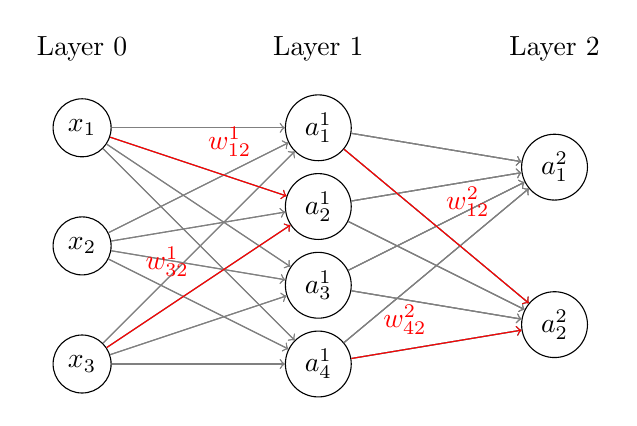
\begin{tikzpicture}
        % layer 0: input layer
        \begin{scope}[name prefix=layer0-]
            \node at (0, 0) {Layer 0};
            \node[circle, draw] (1) at (0, -1) {$x_1$};
            \node[circle, draw] (2) at (0, -2.5) {$x_2$};
            \node[circle, draw] (3) at (0, -4) {$x_3$};
        \end{scope}

        % layer 1
        \begin{scope}[name prefix=layer1-]
            \node at (3, 0) {Layer 1};
            \node[circle, draw] (1) at (3, -1) {$a^1_1$};
            \node[circle, draw] (2) at (3, -2) {$a^1_2$};
            \node[circle, draw] (3) at (3, -3) {$a^1_3$};
            \node[circle, draw] (4) at (3, -4) {$a^1_4$};
        \end{scope}

        % layer 2
        \begin{scope}[name prefix=layer2-]
            \node at (6, 0) {Layer 2};
            \node[circle, draw] (1) at (6, -1.5) {$a^2_1$};
            \node[circle, draw] (2) at (6, -3.5) {$a^2_2$};
        \end{scope}

        % weights
        \foreach \x in {1, 2, 3} {
            \foreach \y in {1, 2, 3, 4} {
                \foreach \z in {1, 2} {
                    \draw[gray, ->] (layer0-\x) -- (layer1-\y);
                    \draw[gray, ->] (layer1-\y) -- (layer2-\z);
                }
            }
        }
        \draw (layer0-1) edge[red, ->] node[auto] {$w^1_{12}$} (layer1-2);
        \draw (layer0-3) edge[red, ->] node[auto] {$w^1_{32}$} (layer1-2);
        \draw (layer1-1) edge[red, ->] node[auto] {$w^2_{12}$} (layer2-2);
        \draw (layer1-4) edge[red, ->] node[auto] {$w^2_{42}$} (layer2-2);
    \end{tikzpicture}
    \end{center}
    \caption{A 2 Layer Neuron Network}
\end{figure}

\subsection{Notations}
\begin{description}
    \item[$L$] output layer.
    \item[$n_l$] number of neurons in layer $l$. In particular, $n_0 = n$.
    \item[$w^l_{ij}$] weight from the $i$-th neuron in the layer $l-1$ to the $j$-th neuron in the layer $l$.
    \item[$b^l_j$] bias of the $j$-th neuron in layer $l$.
    \item[$a^l_j$] activation of the $j$-th neuron in layer $l$.
    \item[$z^l_j$] raw output of the $j$-th neuron in layer $l$.
    \item[$\sigma^l_j$] activation function of the $j$-th neuron in layer $l$.
    \item[$w^l$] weight matrix connecting layer $l-1$ to layer $l$, i.e. $(w^l_{ij})$, of dimension 
    $(n_{l-1},\ n_l)$.
    \item[$b^l$] bias vector of layer $l$, i.e. $(b^l_j)$, of dimension $(1, n_l)$.
    \item[$z^l$] raw output vector of layer $l$, of dimension $(1, n_l)$.
    \item[$a^l$] activation vector of layer $l$, of dimension $(1, n_l)$.
    \item[$\sigma^l$] activation function vector of layer $l$, of dimension $(1, n_l)$.
\end{description}

Some basic equations:

\begin{align}
    z^0_j &= a^0_j = x_j\\
    z^l_j &= \sum_k a^{l-1}_{k} w^l_{kj} + b^l_j\quad\forall~l\geq 1\\
    a^l_j &= \sigma^l_j(z^l_j)
\end{align}
The corresponding matrix forms are:

\begin{align}
    z^0 &= a^0 = \V{x} = (x_1, x_2, \ldots, x_{n})\\
    z^l &= a^{l-1} w^l + b^l\\
    a^l &= \sigma^l(z^l)
\end{align}

For a single input example \V{x}, the cost function $C$ should only directly depend on the output layer $L$,
for example $C$ is the square loss function:
\begin{equation}\label{nn_square_loss}
    C = \frac{1}{2} ||a^L - y||^2_2
\end{equation}
For a collection of examples, the cost function is the average cost on those examples:
\begin{equation}
    C = \frac{1}{m} \sum_{i=1}^m C(\V{x}_i)
\end{equation}

\subsection{Backpropagation}
First let's consider the case with a single input example. Let $\delta^l_j$ be the error in the $j$-th neuron
in the $l$-th layer, i.e.
\begin{equation}\label{delta_l_j}
    \delta^l_j = \pfrac{C}{z^l_j}
\end{equation}

For the output layer $L$, by definition we have:
\begin{align*}
    \delta^L_j &= \pfrac{C}{z^L_j}\\
               &= \sum_k \pfrac{C}{a^L_k} \pfrac{a^L_k}{z^L_j}\\
               &= \pfrac{C}{a^L_j} \pfrac{\sigma^L_j(z^L_j)}{z^L_j}\\
               &= \pfrac{C}{a^L_j}\cdot (\sigma^L_j)'(z^L_j)
\end{align*}
That is,
\begin{equation}
    \delta^L = \nabla_{a^L}C \odot (\sigma^L)'(z^L)
\end{equation}
For example, when $C$ is the square loss~\eqref{nn_square_loss}, $\nabla_{a^L}C = a^L - y$.
\par
We can write $\delta^l$ in terms of $\delta^{l+1}$ as following:
\begin{align*}
    \delta^l_j &= \pfrac{C}{z^l_j}\\
               &= \sum_k \pfrac{C}{z^{l+1}_k} \pfrac{z^{l+1}_k}{z^l_j}\\
               &= \sum_k \delta^{l+1}_k \sum_r \pfrac{a^l_r}{z^l_j} w^{l+1}_{rk}\\
               &= \sum_k \delta^{l+1}_k (\sigma^l_j)'(z^l_j) w^{l+1}_{jk}\\
               &= {\left(\delta^{l+1} \T{(w^{l+1})}\right)}_{j} (\sigma^l_j)'(z^l_j)
\end{align*}
Its corresponding matrix form is:
\begin{equation}
    \delta^l = \left(\delta^{l+1} \T{(w^{l+1})}\right) \odot (\sigma^l)'(z^l)
\end{equation}

Now, let's compute \pfrac{C}{b^l_j}:
\begin{align*}
    \pfrac{C}{b^l_j} &= \sum_k \pfrac{C}{z^l_k} \pfrac{z^l_k}{b^l_j}\\
                     &= \sum_k \delta^l_k \pfrac{b^l_k}{b^l_j}\\
                     &= \delta^l_j
\end{align*}
In shorthand, it can be rewritten as:
\begin{equation}
    \pfrac{C}{b} = \delta
\end{equation}

Similarly, we can compute \pfrac{C}{w^l_{ij}}:
\begin{align*}
    \pfrac{C}{w^l_{ij}} &= \sum_k \pfrac{C}{z^l_k} \pfrac{z^l_k}{w^l_{ij}}\\
                        &= \sum_k \delta^l_k \sum_r \pfrac{(a^{l-1}_r w^l_{rk} + b^l_k)}{w^l_{ij}}\\
                        &= \sum_k \delta^l_k a^{l-1}_i \delta_{kj}\\
                        &= a^{l-1}_i \delta^l_j
\end{align*}
In shorthand, it can be rewritten as:
\begin{equation}
    \pfrac{C}{w} = a_{\text{in}}\delta_{\text{out}}
\end{equation}

For simplicity, let's assume that all the activation functions are the same, i.e. $\sigma^l_i = \sigma$, then 
we can write the pseudocode of backpropagation algorithm easily as the following:

\begin{algorithm}
    \caption{Backpropagation}\label{backpropagation}
    \begin{algorithmic}[1]
        \Require $\V{x} = (x_1, x_2, \ldots, x_n)$
        \For{$l = 1$ \algorithmicto $L$}
            \State Compute $z^l = a^{l-1} w^l + b^l$ and $a^l = \sigma(z^l)$.
        \EndFor
        \State Compute $\delta^l = \nabla_{a^L}C \odot \sigma'(z^L)$\Comment{$\nabla_{a^L}C = a^L - y$ if $C$ 
        is square loss.}
        \For{$l=L-1$ \algorithmicto $1$}
            \State Compute $\delta^l = \left(\delta^{l+1} \T{(w^{l+1})}\right) \odot \sigma'(z^l)$
        \EndFor
        \Ensure $\pfrac{C}{w^l_{ij}} = a^{l-1}_i \delta^l_j$ and $\pfrac{C}{b^l_j} = \delta^l_j$.
    \end{algorithmic}
\end{algorithm}

We are now ready to do the vectorization. Let $\V{x}^i$ and $y^i$
be the $i$-th example and its output respectively, let
\begin{align*}
    X &= {(\V{x}^1; \ldots; \V{x}^m)}_{m \times n}\\
    Y &= {(y^1; \ldots; y^m)}_{m \times n_L}
\end{align*}
the input matrix. 
Let $z^{i, l}, a^{i, l}, \delta^{i, l}$ be the raw output, output, error vectors w.r.t.\ the
$i$-th example respectively. Let 
\begin{align*}
    Z^l &= {(z^{1, l}; \ldots; z^{m, l})}_{m \times n_l}\\
    A^l &= {(a^{1, l}; \ldots; a^{m, l})}_{m \times n_l}\\
    \Delta^l &= {(\delta^{1, l}; \ldots; \delta^{m, l})}_{m \times n_l}
\end{align*}
then we have:
\begin{align}
    Z^l &= A^{l-1} w^l + b^l\\
    A^l &= \sigma(Z^l)\\
    \Delta^L &= \nabla_{A^L}C \odot \sigma'(Z^L)\\
    \Delta^l &= \left(\Delta^{l+1} \T{(w^{l+1})}\right) \odot \sigma'(Z^l)
\end{align}
If $C = \frac{1}{m}\sum_{i=1}^m C(\V{x}_i)$, then
$$\pfrac{C}{b^l_j} = \operatorname{reduce\_mean}(\operatorname{col}_j(\Delta^l))$$
and
$$\pfrac{C}{w^l_{ij}} = \operatorname{reduce\_mean}(\operatorname{col}_i(A^{l-1}) \odot \operatorname{col}_j
(\Delta^l))$$

\subsection{Cost Functions}


\subsection{Regularizations}
\subsubsection{$L^1$ and $L^2$ Regularizations}

\subsubsection{Dropout}

% ========Bayesian Classifier=========
\include{sections/bayesian_classifier}

% ========Expectation Maximalization====
\include{sections/EM}

% ========Ensemble Learning============
\section{Ensemble Learning}

\subsection{AdaBoost}

\begin{algorithm}
    \caption{AdaBoost}\label{AdaBoost}
    \begin{algorithmic}[1]
        \Require training set $D = \{(\V{x}_1, y_1), \ldots, (\V{x}_m, y_m)\}$; base learner $\mathcal{L}$;
        training round $T$.
        \State $\mathcal{D}_1(\V{x}) = \frac{1}{m}$.\Comment{$\mathcal{D}$ is a distribution over the input 
        examples.}
        \For{$t = 1$ \algorithmicto $T$}
            \State $h_t = \mathcal{L}(D, \mathcal{D}_t)$;
            \State $\varepsilon_t = \p_{\V{x}\sim\mathcal{D}_t}(h_t(\V{x})\neq f(\V{x}))$;\Comment{
            $\varepsilon_t$ is the error rate of $h_t$ w.r.t $\mathcal{D}_t$.}
            \State $\alpha_t = \frac{1}{2}\ln{\frac{1 - \varepsilon_t}{\varepsilon_t}}$;
            \State $\mathcal{D}_{t + 1}(\V{x}) = \frac{\mathcal{D}_t(\V{x})\exp(-\alpha_t f(\V{x})h_t(\V{x}))}
            {Z_t}$.\Comment{$Z_t$ is the normalization factor.}
        \EndFor
        \Ensure $H(\V{x}) = \sign(\sum_{t = 1}^T \alpha_t h_t(\V{x}))$
    \end{algorithmic}
\end{algorithm}

% ========Dimension Reduction=========
\section{Dimension Reduction}

\subsection{Low-dimensional embedding}
Let the feature space $\mathcal{X} = \mathbb{R}^d$. Our goal is to find an embedding of all samples into a
low dimension space $\mathbb{R}^{d'}$, here $d' \leq d$. That is, we want to find a map $e: \mathbb{R}^d
\longrightarrow \mathbb{R}^{d'}$ \st for any samples $\V{x}_i, \V{x}_j$, we have 
$$\dist(e(\V{x}_i), e(\V{x}_j)) = \dist(\V{x}_i, \V{x}_j)$$
Thus ${\left\{e(\V{x}_i)\right\}}_i$ is a low-dimensional embedding of the original samples. 

Let $\V{D} = {\left(\dist(\V{x}_i, \V{x}_j)\right)}_{m \times m}$ be the distance matrix of the samples 
${\left\{\V{x}_i\right\}}_i$, we want to find the embedding matrix $\V{Z} \in \mathbb{R}^{m \times d'}$, \st 
$||\V{z}_i - \V{z}_j|| = \V{D}_{ij}$, where $\V{Z} = (\V{z}_1; \dotsc; \V{z}_m)$ and 
$\V{D}_{ij} = \dist(\V{x}_i, \V{x}_j)$. Hence we have 
$$ \V{D}_{ij}^2 = ||\V{z}_i||^2 + ||\V{z}_j||^2 - 2 \langle\V{z}_i, \V{z}_j\rangle$$
Let $\V{B} = {\left(b_{ij}\right)}_{m \times m}= \V{Z}\T{\V{Z}}$ where $b_{ij} = \langle\V{z}_i, \V{z}_j\rangle$, 
we have
\begin{equation}\label{DR_Dij}
    \V{D}_{ij}^2 = b_{ii} + b_{jj} - 2 b_{ij}
\end{equation}
Let $\V{c} = \frac{1}{m}\sum_i \V{z}_i$, then ${\left\{\V{z}_i - \V{c}\right\}}_i$ is an embedding with the
property that $\sum_i(\V{z}_i - \V{c}) = 0$. Hence we can require that $\sum_i \V{z}_i = 0$ in the above
discussion. Then from equation~\eqref{DR_Dij}, we know that:
\begin{align}
    \sum_i \V{D}_{ij}^2 &= \tr(\V{B}) + m b_{jj}\\
    \sum_j \V{D}_{ij}^2 &= \tr(\V{B}) + m b_{ii}\\
    \sum_{i,j} \V{D}_{ij}^2 &= 2m \tr(\V{B})
\end{align}
From the above equations, we have
\begin{equation}\label{DR_bij}
    b_{ij} = -\frac{1}{2}\left(\V{D}_{ij}^2 - \frac{1}{m}\sum_i \V{D}_{ij}^2 - \frac{1}{m} \sum_j \V{D}_{ij}^2
    + \frac{1}{m^2}\sum_{i,j}\V{D}_{ij}^2\right)
\end{equation}
That is, $\V{B}$ is totally determined by $\V{D}$. Let $\V{B} = \V{V}\V{\Lambda}\T{\V{V}}$ be the eigenvalue
decomposition of $\V{B}$. Since $\V{B}$ is semi-positive, $\V{\Lambda}$ is a diagonal matrix with non-negative
diagonals. Let $\V{\Lambda}_*$ be the diagonal matrix obtained by removing the zero eigenvalues from 
$\V{\Lambda}$ and $\V{V}_*$ the matrix by removing the corresponding columns of $\V{V}$. Then it's easy to 
conclude that 
$$\V{Z} = \V{V}_*\V{\Lambda}_*^{\nicefrac{1}{2}}$$
is what we want. Hence the dimension $d'$ is totally determined by the distance matrix $\V{D}$. 

In practise, we often fix some $d' \ll d$ at first, then obtain $\V{\Lambda}_*$ by keeping the $d'$ largest 
eigenvalues and remove the rest, and $\V{V}_*$ the corresponding matrix. By this way, we may lose some 
precision in keeping the pairwise distance, but we can greatly reduce the dimension.

\begin{algorithm}
    \caption{Multiple Dimensional Scaling}
    \begin{algorithmic}[1]
        \Require the distance matrix $\V{D}_{m \times m}$; dimension $d'$.
        \State Compute the matrix $\V{B}$ according to equation~\eqref{DR_bij}.
        \State Eigenvalue decomposition: $\V{B} = \V{V} \V{\Lambda}\T{\V{V}}$.
        \State Let $\V{\Lambda}_*$ be the diagonal matrix with the $d'$ largest eigenvalues and $\V{V}_*$ the
        matrix with the corresponding eigenvectors.
        \Ensure Low-dimensional embedding: $\V{Z} = {\left(\V{V}_* \V{\Lambda}_*^{\nicefrac{1}{2}}\right)}_{m 
        \times d'}$
    \end{algorithmic}
\end{algorithm}

\subsection{Linear Dimension Reduction}
The simplest way to reduce dimension is by dropping some components, that is, via projection.


% ========Computational Learning Theory
\section{Computational Learning Theory}
In this section, we mainly consider supervised learning.
Let $\mathcal{X}$ be the instance space, $\mathcal{Y}$ the label set, $D = \{(\V{x}_1, y_1), \ldots, 
(\V{x}_m, y_m)\}$ the training set. Assume $\mathcal{D}$ is the distribution on $\mathcal{X}$, and all 
instances of $D$ are sampled i.i.d.\ according to $\mathcal{D}$. Let \hypo{f} be the underlying labeling 
function and \hypo{h} any prediction function, then the \textbf{true (generalization) loss (error)} is defined
as:
$$L_{\mathcal{D}, f}(h) := \p_{\V{x}\sim\mathcal{X}}(h(\V{x})\neq f(\V{x})) := \mathcal{D}\left(\{\V{x}: h(\V{x})
\neq f(\V{x})\}\right)$$
the \textbf{empirical risk (error, loss)} is defined as:
$$L_S(h) = \frac{1}{m}\sum_{i=1}^m \indi(h(\V{x})\neq f(\V{x}))$$

\subsection{Probably Approximately Correct Learning}

% concept class.
\begin{df}[Concept class]
    A (target) concept is just a true labeling function \hypo{c}, that is, for any instace $(\V{x}, y)$ 
    (assuming sampling process is noise free) we have $c(\V{x}) = y$. The collection $\mathcal{C}$ of all 
    target concepts is called the concept class.
\end{df}

% hypothesis space.
\begin{df}[Hypothesis space]
    The collection of all labeling functions \hypo{f} a learner $\mathcal{L}$ can return is called the 
    hypothesis space (w.r.t.\ $\mathcal{L}$). We denote it as $\mathcal{H}$.
\end{df}

% inductive bias.
\begin{re}[Inductive bias]
    By restricting our learner to the hypothesis space instead of arbitrary predictors, we bias it toward a 
    particular set of predictors. Such restrictions are called \textbf{inductive bias}.
\end{re}

% realizability assumption.
\begin{df}[Realizability Assumption]
    The realizable assumption asserts that there is a $h^* \in \mathcal{H}$ s.t.\ 
    $L_{\mathcal{D}, f}(h^*) = 0$.
\end{df}

\begin{re}
    The realizable assumption implies that with probability 1 over i.i.d.\ samples $D$, we have $L_D(h^*) = 0$.
    That is, $\mathcal{D}^m(\{D: L_D(h^*) = 0\}) = 1$.
\end{re}

% PAC learnability.
\begin{df}[PAC learnability]\label{PAC_learnability}
    The concept class $\mathcal{C}$ is PAC learnable w.r.t.\ a hypothesis space $\mathcal{H}$ if there exist
    \begin{enumerate}
        \item a function $m: {(0, 1)}^2 \longrightarrow \mathbb{N}$;
        \item a learner $\mathcal{L}$.
    \end{enumerate}
    s.t.\ for any $\varepsilon, \delta \in (0, 1)$, for any distribution $\mathcal{D}$ over $\mathcal{X}$, and
    for any concept \hypo{c}, if the realizable assumption holds w.r.t.\ $\mathcal{H}, \mathcal{D}, c$, then
    when applying the learner $\mathcal{L}$ to $m \geq m(\varepsilon, \delta)$ i.i.d.\ samples generated by
    $\mathcal{D}$ and labeled by $c$, the learner returns a hypothesis $h$ s.t.\ with probability at least 
    $1 - \delta$ (over the choice of the samples), we have $L_{\mathcal{D},c}(h) \leq \varepsilon$. That is,
    $$\mathcal{D}^m(\{D: L_{\mathcal{D},c}(h) \leq \varepsilon\}) \geq 1 - \delta$$
\end{df}

% sample complexity.
\begin{df}[Sample complexity]
    The sample complexity of a learn\-er is the minimal number of examples needed for the learner to produce a 
    PAC solution on any i.i.d.\ data sets with that many samples. That is, it is the minimum of all 
    $m(\varepsilon, \delta)$ where $m$ satisfies the requirements in definition~\ref{PAC_learnability}.
\end{df}

% agnostic PAC learnability.

% ========Reinforcement Learning
\section{Reinforcement Learning}


\end{document}